\documentclass[11pt]{article}

\usepackage{graphicx}
\usepackage{framed}
\usepackage{hyperref}

\marginparwidth 0.5in 
\oddsidemargin 0.25in 
\evensidemargin 0.25in 
\marginparsep 0.25in
\topmargin 0.25in 
\textwidth 6in \textheight 8 in

\begin{document}
\hfill\vbox{\hbox{Jude Shin, Torrey Zachs}
		\hbox{CSC 321, Section 07}	
		\hbox{Module 2: Block Ciphers}	
		\hbox{\today}}\par

\bigskip
\centerline{\Large\bf Lab 02: Symmetric Key Cryptography Exploration}\par
\bigskip

This lab explores symmetric key cryptography security with both Electronic Codebook (ECB) and Cipher Block Chaining (CBC) modes. This lab also demonstrates the limits and exploitations of each, as well as a performance study of public versus symmetric key algorithms. This lab was completed using {\tt Python} and {\tt PyCryptodome}. All the code can be found in our remote \href{https://github.com/jude-shin/CSC\_321}{github} repository.

% ============================================================================
\section*{Environment}

If you want to run and test the code, a virtual environment should first be set up with the correct requirements. This ensures that there is consistency between all of the packages used within this project.

\begin{itemize}
	\item Make a virtual environment (venv) with python.

		\verb|$ python3 -m venv .venv|

	\item Activate the venv.

		\verb|$ source .venv/bin/activate|

	\item Install the requirements using pip.

		\verb|$ pip install -r requirements.txt|

	\item Whenever you are done you can deactivate the venv.

		\verb|$ deactivate|

\end{itemize}

% ============================================================================
\section*{Task 1: Modes of Operation}
\subsection*{Abstract}
The main datatype used was the \verb|bytes| datatype, which could be treated as a fixed array of bytes; this datatype could be iterated over, and indexed, making it easy to locate particular parts of an encrypted or decrypted message. The path to the bmp that the user wants to encrypt is listed as the first command line argument. Both methods of single key encryption use "blocks" of data. In our case, we chose to use 128 but (8 byte) chunk sizes. In our example, we will encrypt some bmp images. In both cases, the first 54 bytes were removed as they were the bmp headers. Then the rest of the data was padded to be divisible by the chosen block size.

\subsection*{Code Breakdown}
\subsubsection*{task1.py}

The python script \verb|task1.py| executes two functions, one to encrypt a file with ECB, and one to encrypt a file with CBC. 

\begin{framed}
\begin{verbatim}
if __name__ == '__main__':
    if len(sys.argv) == 2:
        plaintext_file: str = sys.argv[1]

        encrypt_bmp_with_ecb(plaintext_file)
        encrypt_bmp_with_cbc(plaintext_file)

    else:
        print('One cmd line arg required!')
\end{verbatim}
\end{framed}

\subsubsection*{ECB Code}

The \verb|encrypt_bmp_with_ecb| function will take a filepath for the bmp file, and then open it in bytes. It will then generate a random key; note that this has to be random bytes of the same length as the BLOCK\_SIZE. The data is also padded to the BLOCK\_SIZE. An AES object is used, but the encryption is done only in BLOCK\_SIZEs. We could have used the defined \verb|.encrypt()| functions for this, but for this lab we are choosing to implement the blocks ourself in order to highlight the differences between ECB and CBC methods. Each block that is encrypted is subsequently added to \verb|encrypted_text| variable. Finally, the bmp header is prepended to the encrypted data. The encrypted data is then written to a new file. For testing purposes, the key is also written to a separate file. 

The \verb|decrypt\_ecb| function was implemented with the packages \verb|.decrypt()| function in order to verify that our custom encrypt function was working as intended.

\begin{framed}
\begin{verbatim}
HEADER_SIZE: int = 54
BLOCK_SIZE: int = 16

def encrypt_ecb(text: bytes, key: bytes) -> bytes:
    cipher = AES.new(key=key, mode=AES.MODE_ECB)

    encrypted_text: bytes = b''
    for i in range(0, len(text), BLOCK_SIZE):
        chunk: bytes = text[i:i+BLOCK_SIZE]
        encrypted_text = encrypted_text + cipher.encrypt(chunk)
    return encrypted_text 

def decrypt_ecb(text: bytes, key: bytes) -> bytes:
    # Cipher Function
    cipher = AES.new(key=key, mode=AES.MODE_ECB)
    
    # We can use this library
    return cipher.decrypt(text)

def verify_ecb_encryption(text: bytes, encrypted_text: bytes, key: bytes):
    decrypted_text = decrypt_ecb(encrypted_text, key)
    if (text == decrypted_text):
        print("ecb encryption Verified")
    else:
        print("ecb decrypted value did not match original plain text")

def encrypt_bmp_with_ecb(plaintext_file: str):
    text: bytes | None = read_bytes(plaintext_file)

    key: bytes = random.randbytes(BLOCK_SIZE)
    print(f'key: {key}')
    header: bytes = text[:HEADER_SIZE]
    data: bytes = text[HEADER_SIZE:]
    padded_data: bytes = add_padding(data, BLOCK_SIZE)

    encrypted_text: bytes | None = encrypt_ecb(padded_data, key)
    verify_ecb_encryption(padded_data, encrypted_text, key);

    encrypted_text = header + encrypted_text

    bmp_name = plaintext_file.replace('assets/', '').replace('/', '') \
                             .replace('.bmp', '')
    dir_ = 'encryptions/ecb/'

    write_bytes(dir_ + 'encryption_of_' + bmp_name + '.bmp', encrypted_text)
    write_bytes(dir_ + 'key_of_' + bmp_name + '.txt', key)
\end{verbatim}
\end{framed}

\subsubsection*{CBC Code}

This is almost the same as ECB, however, the previous ciphertext block is first \verb|xor|ed with the current plaintext block before that block is put through the ECB encryption algorithm. This is where the custom implementation of \verb|/encrypt()| becomes more interesting. Before passing the plaintext block into the \verb|.encrypt()| function, we first \verb|xor| it with the previous ciphertext. As for the very first block (which has no "previous" ciphertext), a random initialization vector (IV) is used in it's place. Processing the header and padding follows the same procedure as the ECB encryption. The encrypted file is written to a file. Again, for testing purposes, the Key and IV are written to files as well.

When writing the custom \verb|.encrypt()| function for the CBC method, the AES.MODE had to be specified as \verb|AES.MODE_ECB|. If it \verb|AES.MODE_CBC|, then an IV would automatically be applied every time \verb|.encrypt()| would be called; however, CBC only applies the IV once at the beginning block.

\begin{framed}
\begin{verbatim}
HEADER_SIZE: int = 54
BLOCK_SIZE: int = 16

def encrypt_cbc(text: bytes, key: bytes, iv: bytes) -> bytes:
    # NOTE: if you specify ECB, then it will probably try to use
		# some input vector every time you call encrypt
    cipher = AES.new(key=key, mode=AES.MODE_ECB)

    encrypted_text: bytes = b''
    prev: bytes = iv
    for i in range(0, len(text), BLOCK_SIZE):
        chunk: bytes = text[i:i+BLOCK_SIZE]

        xor: bytes = xor_bytes(chunk, prev)

        prev = cipher.encrypt(xor) 

        encrypted_text = encrypted_text + prev

    return encrypted_text 

def decrypt_cbc(text: bytes, key: bytes, iv: bytes) -> bytes:
    # Cipher Function
    cipher = AES.new(key=key, mode=AES.MODE_CBC, iv=iv)
    
    # We can use this library
    return cipher.decrypt(text)

def verify_cbc_encryption(text: bytes, encrypted_text: bytes,
                          key: bytes, iv: bytes):
    decrypted_text = decrypt_cbc(encrypted_text, key, iv)
    if (text == decrypted_text):
       print("cbc encryption Verified")
    else:
        print("cbc decrypted value did not match original plain text")

def encrypt_bmp_with_cbc(plaintext_file: str) -> None:
    text: bytes | None = read_bytes(plaintext_file)

    # key must be BLOCK_SIZE bytes long (for AES-128)
    key: bytes = random.randbytes(BLOCK_SIZE)
    print(f'key: {key}')

    # iv  must be BLOCK_SIZE bytes long
    iv: bytes = random.randbytes(BLOCK_SIZE)
    print(f'iv: {iv}')
    
    header: bytes = text[:HEADER_SIZE]
    data: bytes = text[HEADER_SIZE:]
    padded_data: bytes = add_padding(data, BLOCK_SIZE)

    encrypted_text: bytes | None = encrypt_cbc(padded_data, key, iv)    
    verify_cbc_encryption(padded_data, encrypted_text, key, iv)

    encrypted_text = header + encrypted_text

    bmp_name = plaintext_file.replace('assets/', '').replace('/', '') \
                             .replace('.bmp', '')
    dir_ = 'encryptions/cbc/'

    write_bytes(dir_+'encryption_of_'+bmp_name+'.bmp', encrypted_text)

    write_bytes(dir_ + 'key_of_' + bmp_name + '.txt', key)
    write_bytes(dir_ + 'iv_of_' + bmp_name + '.txt', iv)
\end{verbatim}
\end{framed}

\subsubsection*{PKCS\#7 Code} 

The PKCS padding scheme adds a number of bytes to the end of the data, ensuring that the encryption algorithm has even blocks to work with. Let the number of remaining bytes that were filled be \verb|k|. Each byte that is appended to the end of the data is the integer \verb|k| represented as a byte. This, of course, is a well defined padding system up to padding of 255 extra bytes.

\begin{framed}
\begin{verbatim}
# pad text bytes with pkcs#7 padding
def add_padding(text: bytes, block_size: int) -> bytes:
    # Get the remainder that is needed to become a multiple of block_size
    k: int = block_size - len(text)%block_size

    # k(byte) will be repeated k times
    single_byte: bytes = k.to_bytes(1, 'big')
    padding: bytes = single_byte * k

    # Append the padding to the end of the text 
    return text + padding 

# remove a padded text bytes with pkcs#7 padding
def strip_padding(text: bytes) -> bytes:
    # Read the last block (should be an int)
    k: int = text[-1]

    # If the number that are in the last k bytes does not match up
		# , then there was no padding (or a padding of 0)
    for i in range(k):
        if (k != text[-(i+1)]):
            return text 

    # Remove the last k bytes in text 
    return text[:-k]
\end{verbatim}
\end{framed}

\subsubsection*{Utilities Code}

Some helper functions were shared between the two encryption methods like reading and writing bytes to a file. Note that we open the file with the binary mode (indicated by the 'b') to indicate that we want a \verb|bytes| datatype instead of a file object.

\begin{framed}
\begin{verbatim}
def read_bytes(filename: str) -> bytes:
    with open(filename, 'rb') as f:
        return f.read()

def write_bytes(filename: str, text: bytes) -> None:
    with open(filename, 'wb+') as f:
        f.write(text)
\end{verbatim}
\end{framed}

\subsection*{Reproduction}

Running both encryption processes on a given bmp is as simple as activating the venv, and then running \verb|task1.py| with the file to be encrypted.

\verb|$ python task1.py ./path/to/image.bmp|

\subsection*{Results and Analysis}

The encrypted BMP images are included below. The ECB encryption (\autoref{fig:ecb}) presents a security flaw: patterns are noticeable and might reveal more information than was intended. Although this is the case, the benefit to this is that the algorithm is robust: it does not rely on previous steps of the encryption process. AES (\autoref{fig:cbc}) is shown to be more obscure because of the \verb|xor| on previous encrypted blocks, but this method allows for errors in previous steps to propagate to the rest of the encryption.

\begin{figure}[!ht]
	\centering
	
\includegraphics[width=0.5\textwidth]{./assets/ecb_encrypted.jpg}
	\caption{A noticeable outline of the Cal Poly logo is shown.}
	\label{fig:ecb}
\end{figure}

\begin{figure}[!ht]
	\centering
	
\includegraphics[width=0.5\textwidth]{./assets/cbc_encrypted.jpg}
	\caption{No useful patterns are shown in this encrypted image.}
	\label{fig:cbc}
\end{figure}

% ============================================================================
\section*{Task 2: Limits of Confidentiality}
\subsection*{Abstract}
\subsection*{Code Breakdown}

The substring that we chose to insert into our function was \verb|'ydmin=true'|. The target string was supposed to include the substring \verb|'addmin=true'| at the very end. Out of the whole concatenated string, the character \verb|'y'| happened to be located at the 21st position in the \verb|bytes| object. The method to byte flip the targeted character involves \verb|xor|ing the target character (in our case 'a') with the plaintext character at that index (in our case 'y'). Finally, we must \verb|xor| that \verb|xor|ed byte one more time: with the byte of the ciphertext in the previous block (exactly BLOCK\_SIZE bytes away from the) index of the character of interest. Note that if we wanted to change a byte in the first block of the message, we would have to know the IV, as in CBC it acts as the "previous" block.

Once we have newly \verb|xor|ed byte, we use it to replace the byte in the original encrypted message at the "previous" block's index.

Full Example: Suppose we have a message that is 16 bytes long. If each block was 8 bytes long, and the byte we wanted to manipulate was at position 10 (it is located at index 2 of the second block), the "previous" byte we would replace would be at index 2 of the original encrypted message.

When the decryption occurs, the bytes before will me scrambled and garbage, however the block with the desired message will contain the new message, with the manipulated byte.

\begin{framed}
\begin{verbatim}
if __name__ == '__main__':
    # The byte we want to flip is at position 21
    text: str = ';ydmin=true'
    mod_char: str = 'y'
    target_char: str = 'a'
    i: int = 21
    ti: int = i - BLOCK_SIZE

    encrypted_text = submit(text)
    decrypted_text = decrypt_cbc(encrypted_text, KEY, IV)

    xor: int = ord(mod_char) ^ ord(target_char)

    modified_byte: bytes = (encrypted_text[ti] ^ xor).to_bytes(1, 'big')
    modified_encrypted_text: bytes = encrypted_text[:ti] + (modified_byte) + encrypted_text[ti+1:]

    print(f'Verification result: {verify(modified_encrypted_text)}')
\end{verbatim}
\end{framed}

\subsubsection*{}
\subsubsection*{}

\subsubsection*{Reproduction}
\subsubsection*{Results and Analysis}


% ============================================================================
\section*{Task 3: Performance Comparison}
\begin{figure}[!ht]
	\centering
	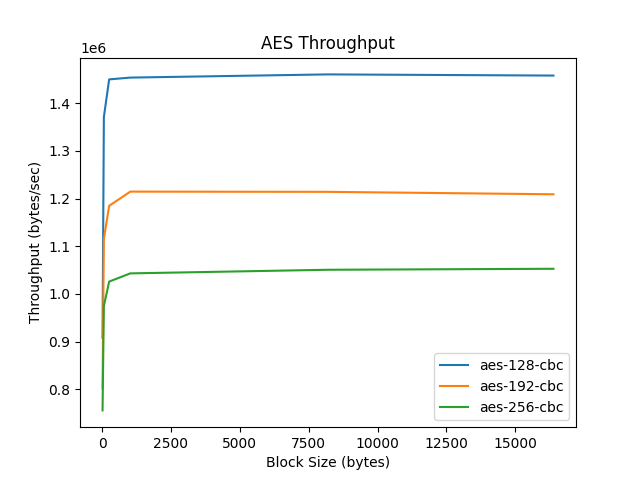
\includegraphics[width=0.5\textwidth]{./assets/aes.png}
	\caption{Throughput of AES}
	\label{fig:aes}
\end{figure}

\begin{figure}[!ht]
	\centering
	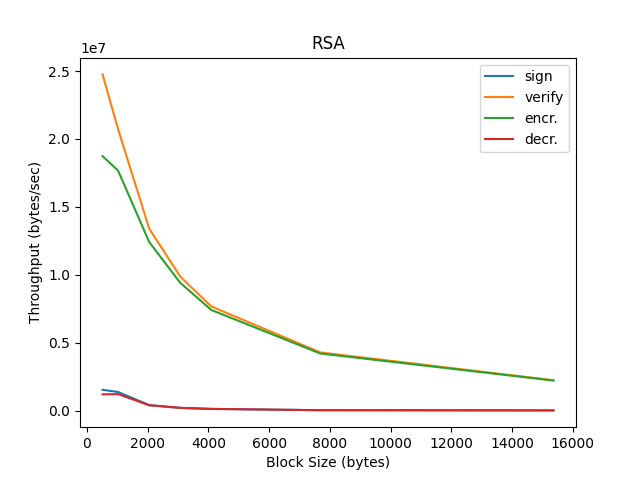
\includegraphics[width=0.5\textwidth]{./assets/rsa.png}
	\caption{Throughput of RSA}
	\label{fig:rsa}
\end{figure}

% ============================================================================
\section*{Questions}
\subsection*{Question 1}

As mentioned before, ECB exposes patterns in the data when looking at the data as a whole; in contrast, CBC offers more obscurity as each block that is encrypted builds on the previous. The encryption compounds in CBC, so even if the same block was encountered in the encryption process, it would be highly unlikely that they would encrypt to the same value. 

\subsection*{Question 2}

This attack is possible because of what CBC uses to try and mask the patterns which arose in the EBC encryption. The block-chain infrastructure builds off of previous encrypted blocks. If the attacker knew some sort of pattern on what the decrypted message may say, they could try and reverse engineer which bits to send through the encryption to modify the output. Authentication methods to ensure that messages have not been tampered with (such as hashing) can prevent these kinds of attacks.

\subsection*{Question 3}

% TODO:

\end{document}
